% =============================================================================
% CHAPTER 3: Methodology (or ``Specification, Design and Implementation'' / ``Approach'')
% =============================================================================
% SPDX-FileCopyrightText: 2026 Frank Langbein <frank@langbein.org>
% SPDX-License-Identifier: LPPL-1.3c
%
% This chapter describes how your solution works. Title it Methodology, Approach,
% or Specification, Design and Implementation; adapt or split as needed. Not all
% sections below apply to every project---pick, omit, or rename.
%
% Suggested sections by project type:
%   System design:  Specification, System design, Implementation. Optional: Datasets
%                   if data is central; Ethical considerations.
%   Research:       Research design, Literature and evidence (search strategy,
%                   inclusion criteria), Specification (= problem + requirements),
%                   Approach and solution, Implementation or experimental setup.
%   AI/ML:          Specification, Datasets, AI/ML models, System design (if a
%                   larger system), Implementation. Optional: Research design,
%                   Literature and evidence; Summary.
% =============================================================================

\newthought{As the proposed solution} of this project is not research-based, appropriate system design took place to keep structure during the development process and to provide quantifiable milestones, aiding in discussion within weekly meetings with the project supervisor.

\section{Specification}\label{sec:spec}
% System design: requirements (what the system must do; optional subsections: functional, non-functional). Research: problem and what is required of a solution.
As discussed in section \ref{sec:related}, it can be observed that each existing device on the market only utilises one input method, whereas the proposed solution needs to listen out for up to three. These methods of input were chosen due to their simple interfaces, the inputs being: terminal commands, physical button interaction and tangible artefact interaction. Simplicity in said input methods can be identified as follows:
\begin{itemize}
    \item The terminal commands are short words part of the English language that describe what they do and are expanded on further using the \texttt{help} command.
    \item The buttons execute one simple command each.
    \item The tangible artefacts require the user to physically tap them against the device, providing a simple physical action the end user needs to perform instead of learning a \gls{ui}.
\end{itemize} 

Before implementation could begin, identifying clear deliverables and subsequent efficiency guidelines had to occur. This was done through the generation of Functional and Non-functional Requirement. These were generated by breaking down what was absolutely necessary for the proposed solution to do and to which degree each of these actions efficiency is necessary.

\subsection{Functional requirements}\label{subsec:funcreq}
To ensure consistency between these modes of input and outlining clear deliverables, the following functional requirements were proposed:
\begin{enumerate}
    \item\label{req:playBtn} Pressing the play/pause button \textbf{must} play and pause the current song being played.
    \item\label{req:skipBtn} Pressing the skip button \textbf{must} skip the current song being played to the next song in the playlist.
    \item\label{req:remoteCon} The device \textbf{must} be able to be interfaced with remotely.
    \item\label{req:correctCommand} Sending commands over a remote terminal \textbf{must} perform the action that it has been assigned to do so.
    \item\label{req:NFCcorrect} Presenting a tangible artifact to the appropriate antenna \textbf{must} perform a playlist switch to a given playlist present on the artefact.
    \item\label{req:audioPlayback} The device \textbf{must} play audio through a predefined speaker.
    \item\label{req:usable} The device \textbf{must} always be in a usable state. 
\end{enumerate}
\subsection{Non-functional requirements}\label{subsec:nonfuncreq}
In a similar vein, the proposed solution needs to function in an efficient and safe manner. It is unreasonable to expect the end users to have to wait extended periods of time for actions to be performed, and potentially compromise their network with the proposed solution as the attacker's entry point. Therefore, the following non-functional requirements were also proposed:
\begin{enumerate}
    \item\label{req:remoteTime} Commands over the remote terminal should take \textbf{no longer than} 5 seconds to execute. Given the simple nature of the commands passed into the terminal, the expectation of response time will likely be instant, although expectations may vary \citep{shneiderman1984response}.  
    \item\label{req:remoteAuth} Users without authorisation should \textbf{not} be able to connect to the device remotely, ensuring the security of the device.
    \item\label{req:easeofuse} The device needs to be \textbf{intuitive} and easy to use.
    \item\label{req:startupTime} Start-up of the device should take \textbf{no longer than} 2 minutes. This is based off experience throughout development on the Raspberry Pi on its average boot times and what the author expects to be the average expectation for boot times.
    \item\label{req:NFCtolerance} The device should read a presented tangible artifact successfully in \textbf{no more than} 10 attempts. This provides a reasonable buffer identifying if the data collection delay is a hardware/software fault or due to user error.
    \item\label{req:scalability} The device should be \textbf{scalable}, and not suffer any performance drops as the playlists increase in size.
    \item\label{req:reboot} The device should \textbf{reboot} after a power cut and return to a \textbf{workable state} once power is restored.
\end{enumerate}

\section{AI and machine learning models}\label{sec:aiml}
% AI/ML: model choice, training and validation, evaluation methodology. Omit otherwise.
Although not instrumental to the design, AI chatbots powered by \gls{llm}s were utilised throughout the development of this project. These \gls{llm}s were used in a supportive capacity, largely through troubleshooting code or brainstorming ideas on how to execute potential features, in particular the utilisation of Python Sockets to execute terminal commands. Each piece of code produced by these models were thoroughly examined and rigorously tested to ensure it was efficient, no vulnerabilities were present and to further the understanding of the author as to what the code intends to do. The code was then rewritten and adapted to a particular use case.

The \gls{llm}s utilised for this project are the following:
\begin{itemize}
    \item Claude by Anthropic \citep{Anthropic2026}.
    \item Gemini by Google \citep{GoogleAI2026}.
    \item Microsoft Copilot by Microsoft AI and OpenAI \citep{MicrosoftAI2026}.
\end{itemize}

\section{System design}\label{sec:design}
% System design: architecture, data flow, behaviour (UML, ER, state charts). Use diagrams. Research: use ``Approach and solution'' for your proposed solution(s).
The system has been designed around three main hardware components:
\begin{enumerate}
    \item \texttt{Raspberry Pi 4 Model B}
    \item \texttt{Arduino Expansion Shield} acting as an Arduino Leonardo board
    \item \texttt{Bluetooth Speaker} in this case, a Google Nest Mini.
\end{enumerate}
However, the Raspberry Pi and Arduino Board are connected unconventionally, due to a GrovePi+ being already attached to the header pins of the Raspberry Pi. They are instead connected through a USB port on the Raspberry Pi itself. The Arduino is necessary here to connect the \gls{nfc} Reader Module, as its Base Shield possesses a UART connection, that the GrovePi+ does not have access to. A detailed diagram of how these components are connected with all accompanying sensors, buttons and speakers can be seen in Figure \ref{fig:sysoverH}.

\begin{figure}[H]
  \centering
  \fbox{\rule{0pt}{4cm}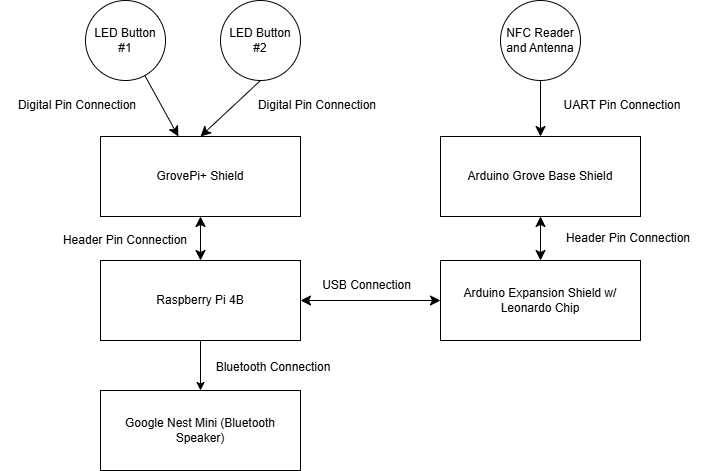
\includegraphics[width=0.97\textwidth]{images/SystemOverviewHardware}}
  \caption[System Overview - Hardware]{System Overview - Hardware}\label{fig:sysoverH}
\end{figure}

The software this project consists of can be separated into 3 main scripts:
\begin{enumerate}
    \item \texttt{client.py}, used for sending commands to the main program.
    \item \texttt{server.py}, housing the core functionality of the media player and receiving commands from both the Arduino and \texttt{client.py}.
    \item \texttt{reading\_nfc.ino}, used for reading the data off \gls{nfc} tags.
\end{enumerate}
This separation was necessary due to factors revolving around how UNIX sockets work between programs (necessitating the separation for communication to occur) and different systems requiring different programming languages (in this case, the Arduino running scripts in C++).  

An additional script for the Arduino also exists called "\texttt{writing\_nfc.ino}" but it is only necessary when creating new \gls{nfc} tags for new or existing playlists. A detailed diagram of how these interact with each other can be seen in Figure \ref{fig:sysoverS}.

\begin{figure}[H]
  \centering
  \fbox{\rule{0pt}{4cm}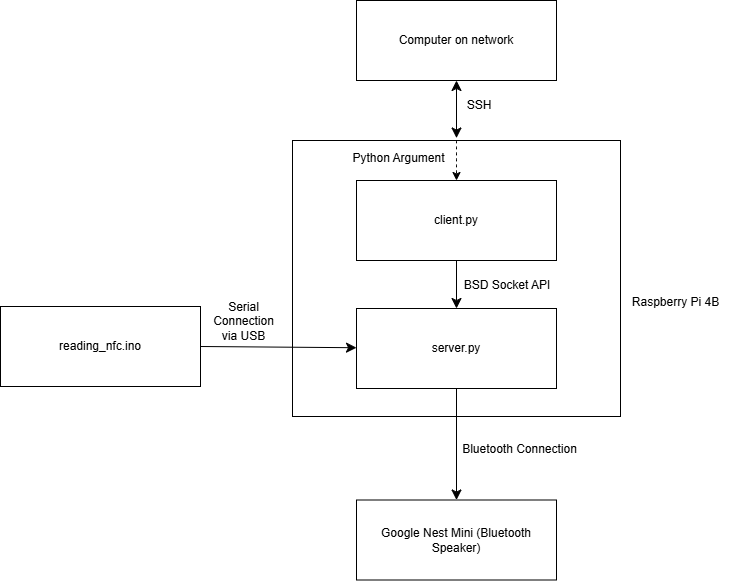
\includegraphics[width=0.97\textwidth]{images/SystemOverviewSoftware}}
  \caption[System Overview - Software]{System Overview - Software}\label{fig:sysoverS}
\end{figure}

The Python scrips utlises 2 external libraries to execute all of its functions, the rest being included in a Python 3 installation. The list of the libraries and what they were for is as follows:
\begin{itemize}
    \item grovepi, one of the external libraries that allows for direct interaction with the pins on the GrovePi+ shield.
    \item python-vlc, the other external library that allows for the music to be played through Raspbian's default media player VLC. Controls for the songs are managed through this library.
    \item time, a native Python library that introduced delays in the scripts, allowing for Bluetooth connection to occur without disruption.
    \item threading, a native Python library that allowed for multiple functions (in this case, reading \gls{nfc} tags and receiving terminal commands) to run concurrently.
    \item socket, a native Python library that utilises the BSD Socket API to communicate between \texttt{server.py} and \texttt{client.py}.
    \item subprocess, a native Python library that allowed for execution of terminal commands (in this case, bluetoothctl).
    \item os, a native Python library that read all of the song files in a given directory to construct a playlist.
    \item serial, a native Python library that facilitated reading from the serial port. 
    \item re, a native Python library that could enact regular expressions on the payloads of the \gls{nfc} tags.
    \item random, a native Python library that facilitated the "shuffle" functionality in the media player.
\end{itemize}

The C++ sketches for the Arduino utilised a library provided by Seeed Studios to interface with the \gls{nfc} reader, using \gls{ndef} formatting \citep{SeeedStudios2020}.

A full list of the hardware that was used in this project is the following:
\begin{itemize}
    \item \texttt{Raspberry Pi 4 Model B}
    \item \texttt{MicroSD Card 32Gb}
    \item \texttt{GrovePi+ Shield}
    \item \texttt{2 Grove LED Buttons}
    \item \texttt{Arduino Expansion Shield for Raspberry Pi B+ (V2.0)}
    \item \texttt{Grove Base Shield for Arduino}
    \item \texttt{Grove \gls{nfc} Reader}
    \item \texttt{5 \gls{nfc} tags}
    \item \texttt{Google Nest Mini}
    \item \texttt{Laptop} capable of \gls{ssh}
\end{itemize}

\section{Ethical considerations}\label{sec:ethics}
Dealing with a protected characteristic such as disability means ethics is rooted deeply within this project. To be able to user test with the stakeholders, full ethics approval is required. Given the timescale of this project, this was not feasible. 

The author instead opted to omit meeting the stakeholders directly, and in their stead, work with carers in the field instead. An argument can be made that since the author's intention was to communicate with private care homes with the assistance of ENRICH Cymru, simplified ethics could still be applied as they are not NHS staff.

For the sake of simplicity, the decision to include workers was also scrapped. Had more time and resources be allocated towards this project, researchers in the field would instead be the subject of user tests to hopefully provide actionable feedback on the proposed solution.

\section{Implementation}\label{sec:impl}
% Realisation: key implementation choices and critical code; avoid describing every module. Optional: tools, platform, problems encountered.
The goal of the implementation was to create each feature of the proposed solution one at a time, ensuring each feature worked in isolation before it was implemented to the system at large. The device was prepped with the prerequisites for working with the given peripherals and the following features were developed in order:
\begin{itemize}
    \item Button interaction was developed for the Grove LED Buttons.
    \item Music Player functionality was mapped to the buttons.
    \item Terminal interaction was developed through Python Sockets.
    \item Start-up behaviour was configured and scripts amended to accommodate it.
    \item \gls{nfc} interaction was developed on an Arduino and integrated into the system.
\end{itemize} 

\subsection{Initial Setup}\label{subsec:setup}
Producing a device that has been designed for mass rollout, a consistent and stable development environment was of paramount importance. It needed to be reproducible, so all units could have the same underlining technologies, and able to communicate with the modules used to interface with the device. To achieve this goal, all the appropriate libraries for the GrovePi library to work were installed on the most current image that supported the peripherals.

Incompatibilities throughout development helped inform this choice. They ranged from deprecated libraries within an older OS version, such as \texttt{easy\_install}, to the OS kernel itself and the underlying frameworks for communication over the \gls{i2c} interface \citep{IOTGarage2025}.

The GrovePi+ itself and its accompanying software and libraries helped identify each of these dependencies. Correct Raspberry Pi OS image choice went on to highlight the importance of the development environment as a whole, rather than in terms of package incompatibilities. This was largely due to the GrovePi+ also being a peripheral that has since been discontinued \citep{PiHut} so continued support from the manufacturer had ceased at the time of the development of the proposed solution.

The pre-configured image provided by Dexter Industries for the GoPiGo family of robots was considered as a potential candidate for the operating system \citep{DexterIndustriesGoPiGo2026} but after examining the image, it was not suitable for the use case, being bloated with unnecessary applications and local web server hosting that would waste system resources when running idle.

The importance of the open-source community helped drive the image choice as the kernel incompatibility \citep{cyclicalobsessive2024} and countless other nuances of other images (such as lacking appropriate public keys for \texttt{apt update} \citep{Jean2026} and outdated source lists in \texttt{/etc/apt/sources.list} \citep{rpdom2026}) were identified through community driven web-forums.

The decision to follow a guide provided by IOT Garage \citep{IOTGarage2025} and the installation of the \texttt{2024-10-22-raspios-bullseye} image was made, which is the current image on the proposed solution. This provided a compromise for currency of the image and having the appropriate OS kernel and \gls{i2c} communication framework. The only deviation from the guide is the copying of both the \texttt{di\_i2c} and \texttt{di\_mutex} modules (they both depend on each other) into the Python 3.9 directory.
\begin{fullwidthfigure}[H]
  \centering
  \fbox{\rule{0pt}{2cm}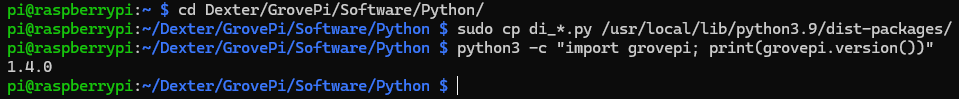
\includegraphics[width=0.97\linewidth]{images/workinggpi}}
  \caption[Movement of Modules and Test grovepi call]{Movement of Modules and Test grovepi call}\label{fig:workinggpi}
\end{fullwidthfigure}

The initial setup was now complete and development of the solution could commence. Although time-consuming, the initial setup helped highlight the idiosyncrasies of working on embedded systems. In a final system, working with peripherals that interfaced directly with the Raspberry Pi's \gls{gpio} pins would be prioritised instead. This would mitigate software dependencies as no third-party libraries would be necessary for interfacing with all of the peripherals, as the core library \texttt{GPIOZero} comes pre-installed on the latest Raspberry Pi Images \citep{bennuttal2024}. 

\subsection{Button Interaction}\label{subsec:btnint}
The proposed solution's main form of interaction is that of button presses on the Raspberry Pi. Once the GrovePi library was installed, focus was put on ensuring that button presses were recognised by the main Python script, using the GrovePi library.

Many of the Grove peripherals contained 2 ports in terms of addressing them and their properties. Working with these peripherals helped highlight how each proprietary module may have its own numbering convention on which port is assigned to what attribute of the peripheral. This was pivotal in the case of the Grove LED buttons where the addressing of the inputs was \textbf{offset by 1}. This was identified through the testing of the original port number and introducing the offset in algorithm \ref{alg:goodBtnTest}.

\begin{algorithm}[H]
    \caption{Successful Button Port Test - Python}
    \label{alg:goodBtnTest}
    \begin{lstlisting}[language=Python]
    import time
    import grovepi

    buttonP_pin = 3 # Port number + 1 recognises button input
    buttonS_pin = 8

    grovepi.pinMode(buttonP_pin, "INPUT")
    grovepi.pinMode(buttonS_pin, "INPUT")

    print("Ready!")
    \end{lstlisting}
\end{algorithm}
The offset identified was counterintuitive, as the labeling on the GrovePi+ shield was sequential, but the address for the button input was one higher. This quirk was not accurately described in the documentation provided the manufacturer and could cause potential issues with peripherals connected sequentially. 

\subsection{Music Player Functionality}\label{subsec:playlist}
Once the button presses were being recognised, music player functionality was implemented. This would include mapping button presses to their appropriate actions and loading a scalable playlist with a series of music files, with the possibility to shuffle them.

The python-vlc package was installed to interface with VLC, which acted as the media player for the proposed solution. It was chosen due to its universality of outputting various media files and open-source nature. Adaptations were made to the main script to map python-vlc's functions to the appropriate button presses, present in Algorithms \ref{alg:initVLC} and \ref{alg:mappedBtnPress}.

\begin{algorithm}[H]
  \caption{Initialisation of VLC Playlist - Python}
  \label{alg:initVLC}
  \begin{lstlisting}[language=Python]
    media_player = vlc.MediaListPlayer() # Intialises Playlist
    instance = vlc.Instance() # Creates VLC instance

    playlist = instance.media_list_new()

    for sound in os.listdir("AudioTracks"): # Creates a Playlist for all audio tracks in /AudioTracks/
        media = instance.media_new(f'AudioTracks/{sound}')
        playlist.add_media(media)

    media_player.set_media_list(playlist)
  \end{lstlisting}
\end{algorithm}
The MediaListPlayer here abstracts the entirety of the indexing of the music files, opting for a 'Black Box' solution, where each song within the \texttt{media\_list} is a separate object that cannot be interacted with directly. Instead, methods provided by python-vlc have to be utilised, as seen in algorithm \ref{alg:mappedBtnPress}.

\begin{algorithm}[H]
  \caption{Mapped Button Presses - Python}
  \label{alg:mappedBtnPress}
  \begin{lstlisting}[language=Python]
    buttonS_was_pressed = False
    buttonP_was_pressed = False
    while True:
        buttonP_state = grovepi.digitalRead(buttonP_pin)
        buttonS_state = grovepi.digitalRead(buttonS_pin)
        
        if buttonP_state == 0 and not buttonP_was_pressed:
            media_player.pause()
            buttonP_was_pressed = True
            
        if buttonS_state == 0 and not buttonS_was_pressed:
            media_player.next()
            buttonS_was_pressed = True
            
        if buttonS_state == 1 and buttonS_was_pressed:
            buttonS_was_pressed = False  
        elif buttonP_state == 1 and buttonP_was_pressed:
            buttonP_was_pressed = False

        time.sleep(0.05)
  \end{lstlisting}
\end{algorithm}
Interestingly, separate pause and play logic was not necessary to implement as the \texttt{vlc.MediaListPlayer} pause function acts as a toggle and pauses or plays respective of the current state of the player. The buttons actions have now been mapped with their designated actions.

To adjust for scalability and the implementation of more than one playlist, the function responsible for this was moved into a dedicated Python function. This was done for modularity and avoiding repeating code when a playlist is to be switched. It takes two arguments, the playlist name and a shuffle boolean. If shuffle is not passed, it defaults to False. The code snippet can be seen in Algorithm \ref{alg:loadplaylist}.
\begin{algorithm}[H]
  \caption{load\_playlist() - Python}
  \label{alg:loadplaylist}
  \begin{lstlisting}[language=Python]
    def loadplaylist(playlistName, shuffle="false"):
        if playlistName == '':
            return False
        
        try:
            os.listdir(f'AudioTracks/{playlistName}')
        except FileNotFoundError:
            return False
        
        playlist = instance.media_list_new()
        
        if shuffle.lower() == "true":
            songs = os.listdir(f'AudioTracks/{playlistName}')
            random.shuffle(songs)
            for sound in songs:
                print(sound)
                media = instance.media_new(f'AudioTracks/{playlistName}/{sound}')
                playlist.add_media(media)
        else:
            for sound in sorted(os.listdir(f'AudioTracks/{playlistName}')):
                print(sound)
                media = instance.media_new(f'AudioTracks/{playlistName}/{sound}')
                playlist.add_media(media)
        media_player.set_media_list(playlist)
        return True
  \end{lstlisting}
\end{algorithm}
This function is able to discern between valid inputs and returns either a True if a playlist switch has successfully occured or a False if an error was caught (either through the playlist not existing or a null value being inputted). This provides a lightweight version of error checking that helped streamline the testing process, as seen in algorithm \ref{alg:playlistTest}. 

This section helped illustrate the importance of reading documentation of an external library and how its dedicated data structures could be interfaced with.
\subsection{Terminal Interaction}\label{subsec:terminal}
% % GOAL
% Create terminal solution that can be interfaced using SSH
% % APPROACH
% UNIX Socket with client/server model
% % KEY DECISIONS/FINDINGS
% systemd gives no terminal

Remote Management was one of the key aims for this project and without the presence of a GUI to facilite this requirement, terminal commands were introduced. The approach taken for terminal interaction was utilising Python's \texttt{socket} library, creating a socket network architecture. 

The "remote" aspect for the Remote Management came from connecting to the device using \gls{ssh} and interfacing with the terminal provided from the connection, as example of such can be seen in Figure \ref{fig:sshEg}. \gls{ssh} was chosen as the remote solution as it is lightweight on a system, with the OpenSSH server not visibly impacting performance, and due to its security, requiring a key exchange at initial connection and credentials for each login attempt. Alternatives for remote management were also explored, such as \gls{vnc} with a desktop environment but a terminal window is still required.

\begin{fullwidthfigure}[H]
  \centering
  \fbox{\rule{0pt}{1.3cm}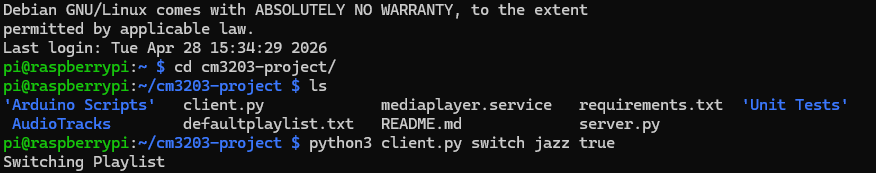
\includegraphics[width=0.97\linewidth]{images/sshExample}}
  \caption[SSH Example]{SSH Example - Switching Playlists}\label{fig:sshEg}
\end{fullwidthfigure}

Given the development context of the proposed solution, where \texttt{systemd} is utilised for running the main script on start-up, the socket architecture was chosen to send and receive commands via Python files, allowing for any \gls{ssh} session and terminal to interface with the device. A simpler approach was originally setup through the use of a \texttt{While True} loop executing in tandem with the button recognition commands, using the \texttt{threading} library, but the lack of an attached terminal ruled out this approach. Anthropic's \gls{llm} Claude was able to assist here, originally suggesting the utilisation of sockets, which it later drafted an implementation for \citep{AnthropicMarch2026}. 

The commands the user has at their disposal are:
\begin{itemize}
    \item play/pause, represented as "p"
    \item skip, represented as "s"
    \item switch, allowing the user to switch to the playlist passed as an argument
    \item help, providing a menu on what each command does 
\end{itemize}

Using a UNIX socket, a secondary smaller script \texttt{client.py} would send a message to \texttt{main.py} (now being renamed \texttt{client.py}) to decode and execute the command the message contained. The socket receiver now also needed to run in tandem, so it became the 2\textsuperscript{nd} thread and was executed using the \texttt{threading} library.

The 2 Python facilitating the communication over the socket architecture \texttt{client.py} and \texttt{server.py} can be seen in Algorithms \ref{alg:clientpy} and \ref{alg:socketReceiverSnip}.
\begin{algorithm}[H]
  \caption{client.py - Python}
  \label{alg:clientpy}
  \begin{lstlisting}[language=Python]
    import socket
    import sys

    def send_command(command):
        if command == '':
            return "Invalid command\n"
        
        socket_path = '/tmp/musicplayer.sock'
        client = socket.socket(socket.AF_UNIX, socket.SOCK_STREAM)
        client.connect(socket_path)
        
        client.send(command.encode())
        response = client.recv(1024).decode()
        client.close()
        return response

    if __name__ == '__main__':
        command = ' '.join(sys.argv[1:])
        response = send_command(command)
        print(response)
  \end{lstlisting}
\end{algorithm}
\texttt{client.py} takes the arguments that have been passed alongside its execution and encodes them to send over the UNIX socket. The response is limited to 1024 bytes due to them being simple enough, anymore would be unnecessary. This can be easily amended should more complex functionality be implemented.

\begin{algorithm}[H]
  \caption{terminal\_server() Snippet - Python}
  \label{alg:socketReceiverSnip}
  \begin{lstlisting}[language=Python]
    def terminal_server():
        server = socket.socket(socket.AF_UNIX, socket.SOCK_STREAM)
        socket_path = '/tmp/musicplayer.sock'
        if os.path.exists(socket_path):
            os.remove(socket_path)
        server.bind(socket_path)
        server.listen(1) # Listens out to only one command  
        while True:
            conn, _ = server.accept()
            data = conn.recv(1024).decode().strip()
  \end{lstlisting}
\end{algorithm}
To ensure that the clean-up process has been executed, \texttt{terminal\_server()} checks if the socket path already exists and deletes it if it remains. This ensures that the current socket has not impacted by previous commands that may have been passed prior to the execution of \texttt{client.py}.

The device could now receive terminal commands through any \gls{ssh} terminal. This section was able to bring light to how two separate Python scripts are able to interact with each other, simulating a network connection through the use of Python's \texttt{socket} library.
\subsection{Start-up Behaviour}\label{subsec:startup}
The device should not need remote interaction on start-up. If this was to be omitted, this would overcomplicate the device and make it inferior to devices already on the market, where simplicity thrives. Remote Management should be an add-on, rather than a necessary tool. The device therefore needed to start playing music the moment it turns on, or reboots after a power cut. This was done through the use of \texttt{systemd} on the Raspberry Pi, where a service was created that would run \texttt{server.py}.

Algorithm \ref{alg:playerServ} shows how \texttt{mediaplayer.service} file utilised in \texttt{systemd}. This service was moved to \texttt{/etc/systemd/system/} and activated using \texttt{systemctl start mediaplayer.service} resulting in it being executed each time the Raspberry Pi reboots. 
\begin{algorithm}[H]
  \caption{mediaplayer.service}
  \label{alg:playerServ}
  \begin{lstlisting}
    [Unit]
    Description=Music Player
    After=network.target sound.target

    [Service]
    ExecStart=/usr/bin/python3 /home/pi/cm3203-project/server.py
    WorkingDirectory=/home/pi/cm3203-project
    User=pi
    Environment=XDG_RUNTIME_DIR=/run/user/1000
    Restart=on-failure
    RestartSec=5

    [Install]
    WantedBy=multi-user.target
  \end{lstlisting}
\end{algorithm}
The utilisation of \texttt{Environment=XDG\_RUNTIME\_DIR=/run/user/1000} here ensures that the user has logged on, which happens automatically on start-up. It specifically double checks if the user session buffer has been created, ensuring VLC and PulseAudio are running, which \texttt{client.py} is dependent on. 

As the device utilises a Bluetooth speaker to play the desired media, the Bluetooth device needed to be paired on start-up as well. This was ensured through a function in \texttt{server.py} that executes before the main script does. It attempts to connect to a given MAC address of a Bluetooth device a total of 10 times, before it times out. This time-out then allowed for support to be carried out by a carer to connect a Bluetooth device manually. 

To ensure that some music is also played on start-up, the \texttt{load\_playlist()} function was called with a text file called \texttt{defaultplaylist.txt} that the end user is free to amend to a different playlist.

This section demonstrated how modern Linux systems execute programs on start-up through \texttt{systemd} through the utilisation of \texttt{.service} files.
\subsection{NFC Reading and Command Execution}\label{subsec:NFC}
As time allowed during the development of this project, tangible item interaction utilising \gls{nfc} was implemented alongside the button interaction. This was done through connecting the Raspberry Pi and an Arduino with the \gls{nfc} module attached to a \gls{uart} connection. These two devices were then connected over a USB, with the Raspberry Pi reading the output from the serial port of the USB bus.

The Arduino had two sketches, one for writing to the \gls{nfc} tags (Algorithm \ref{alg:writeNFC}) and one for reading them (Algorithm \ref{alg:readNFC}). Both scripts were adapted from sketches provided from the IOT Garage Lab Book GitLab \citep{Perera2024} and included a library to be able to interface with the module on the Arduino \citep{SeeedStudios2020}.

\begin{algorithm}[H]
  \caption{writing\_nfc.ino - C++}
  \label{alg:writeNFC}
  \begin{lstlisting}[language=C++]
    #include <NfcAdapter.h>
    #include <PN532/PN532_HSU/PN532_HSU.h>

    PN532_HSU pn532hsu(Serial1);
    NfcAdapter nfc(pn532hsu);

    String record_entry = "NAME_OF_PLAYLIST";

    void setup() {
        Serial.begin(9600);
        while(!Serial);
        Serial.println("NDEF Writer");
        nfc.begin();
    }

    void loop() {
        if (nfc.tagPresent()) {
            Serial.println("NFC TAG FOUND");
            NdefMessage message = NdefMessage();

            message.addUriRecord(record_entry);

            bool success = nfc.write(message);
            
            if (success) {
                Serial.println("Write succeeded.");
            } else {
                Serial.println("Write failed.");
            }
        }
    }
  \end{lstlisting}
\end{algorithm}

\begin{algorithm}[H]
  \caption{reading\_nfc.ino - C++}
  \label{alg:readNFC}
  \begin{lstlisting}[language=C++]
    #include <NfcAdapter.h>
    #include <PN532/PN532_HSU/PN532_HSU.h>

    PN532_HSU pn532hsu(Serial1);
    NfcAdapter nfc(pn532hsu);

    void setup() {
        Serial.begin(9600);
        while(!Serial);
        Serial.println("NDEF Reader");
        nfc.begin();
    }

    void loop() {
        if (nfc.tagPresent()) {
            NfcTag tag = nfc.read();
            tag.print(); // Prints to serial port
        }
        delay(1000);
    }
  \end{lstlisting}
\end{algorithm}

Once the tags have been written and been presented to the \gls{nfc} module, \texttt{server.py} extracted the information using Regular Expressions from the serial output of the USB bus, located through executing \texttt{ls} in \texttt{/dev/} \citep{Quibits2026}, and switches playlists based off the payload passed on the \gls{nfc} tag, as seen in Algorithm \ref{alg:readNFCPy}.

\begin{algorithm}[H]
  \caption{nfc\_reader\_switch() - Python}
  \label{alg:readNFCPy}
  \begin{lstlisting}[language=Python]
    #Accepting NFC Tags
    serial_port = '/dev/ttyACM0'
    baud_rate = 9600

    ser = serial.Serial(serial_port, baud_rate)
   
    while True:
        serData = ser.readline().decode('utf-8', errors='ignore')
        if serData.startswith("    Payload"):
            if serData.startswith("    Payload L") == False:
                print(serData)
                pattern = r'\.([a-zA-Z]+(?:\s+[a-zA-Z]+)?)'
                message = re.findall(pattern, serData) 
                if len(message) == 0:
                    print('Error reading NFC tag, attempt again...')
                else:
                    split_msg = message[0].split()
                    media_player.stop()
                    if len(split_msg) > 1:
                        loadplaylist(split_msg[0], split_msg[1])
                    else:
                        loadplaylist(message[0])
                    media_player.play()

  \end{lstlisting}
\end{algorithm}
The regular expression here extracts exactly the information that is needed from the NFC tag, given its formatting. Most of the data provided by scanning the NFC tag is unnecessary for the application for the proposed solution, so is omitted through checking for the desired line that carries the payload.

This section demonstrated how two separate embedded systems are able to communicate with each other, using a common interface as an intermediary (in this case, the serial port).

\section{Summary}\label{sec:summary}
% Optional: short summary of the methodology. Omit if the chapter is already concise.
The methodology for this project aimed to tackle each feature individually on a weekly basis, as proposed by the initial project plan. These features were:
\begin{enumerate}
    \item Set up the Raspberry Pi with GrovePi and all the necessary libraries.
    \item Implement button interaction so Raspberry Pi recognises input.
    \item Implement media player functionality with buttons and terminal interaction.
    \item Set up start-up behaviour so music player plays automatically.
    \item Implemenet \gls{nfc} interaction to switch playlists.
\end{enumerate}
This methodology remained fluid throughout development as no strict deadlines were imposed for the creation of these features. The methodology will be discussed more in depth in section \ref{sec:discussion}.